\documentclass[a4paper, 11pt]{article}

%Math
\usepackage{amsmath}
\usepackage{amsfonts}
\usepackage{amssymb}
\usepackage{amsthm}
\usepackage{ulem}
\usepackage{stmaryrd} %f\UTF{00FC}r Blitz!

%PageStyle
\usepackage[ngerman]{babel} % deutsche Silbentrennung
\usepackage[ansinew]{inputenc} % wegen deutschen Umlauten
\usepackage{fontenc}
\usepackage{fancyhdr, graphicx} %for header/footer
\usepackage{wasysym}
\usepackage{fullpage}
\usepackage{textcomp}

% Listings
\usepackage{color}
\usepackage{xcolor}
\usepackage{listings}
\usepackage{caption}

% Code listenings
\DeclareCaptionFont{white}{\color{white}}
\DeclareCaptionFormat{listing}{\colorbox{gray}{\parbox{\textwidth}{#1#2#3}}}
\captionsetup[lstlisting]{format=listing,labelfont=white,textfont=white}
 
\lstdefinestyle{JavaStyle}{
 language=Java,
 basicstyle=\footnotesize\ttfamily, % Standardschrift
 numbers=left,               % Ort der Zeilennummern
 numberstyle=\tiny,          % Stil der Zeilennummern
 stepnumber=5,              % Abstand zwischen den Zeilennummern
 numbersep=5pt,              % Abstand der Nummern zum Text
 tabsize=2,                  % Groesse von Tabs
 extendedchars=true,         %
 breaklines=true,            % Zeilen werden Umgebrochen
 frame=b,         
 %commentstyle=\itshape\color{LightLime}, Was isch das? O_o
 %keywordstyle=\bfseries\color{DarkPurple}, und das O_o
 basicstyle=\footnotesize\ttfamily,
 stringstyle=\color[RGB]{42,0,255}\ttfamily, % Farbe der String
 keywordstyle=\color[RGB]{127,0,85}\ttfamily, % Farbe der Keywords
 commentstyle=\color[RGB]{63,127,95}\ttfamily, % Farbe des Kommentars
 showspaces=false,           % Leerzeichen anzeigen ?
 showtabs=false,             % Tabs anzeigen ?
 xleftmargin=17pt,
 framexleftmargin=17pt,
 framexrightmargin=5pt,
 framexbottommargin=4pt,
 showstringspaces=false      % Leerzeichen in Strings anzeigen ?        
}

%Config
\renewcommand{\headrulewidth}{0pt}
\setlength{\headheight}{15.2pt}
\pagestyle{plain}

%Metadata
\title{Algorithmen \& Datenstrukturen 2}
\author{Jan F�ssler}
\date{3. Semester (HS 2012)}
\fancyfoot[C]{If you use this documentation for a exam, you should offer a beer to the authors!}

% hier beginnt das Dokument
\begin{document}

% Titelbild
\maketitle
\thispagestyle{fancy}

\newpage

% Inhaltsverzeichnis
\pagenumbering{Roman}
\tableofcontents	  	


\newpage
\setcounter{page}{1}
\pagenumbering{arabic}

% Inhalt Start

\section{Listen}
Eine verkettete Liste (linked list) ist eine dynamische Datenstruktur zur Speicherung von Objekten. Sie eignen sich f�r das speichern einer unbekannten Anzahl von Objekten, sofern kein direkter Zugriff auf die einzelnen Objekte ben�tigt wird. Jedes Element in einer Liste muss neben den Nutzinformationen auch die notwendigen Referenzen zur Verkettung enthalten.\\ 
Es gibt drei verschiedene Arten von Listen:\\
\begin{center}
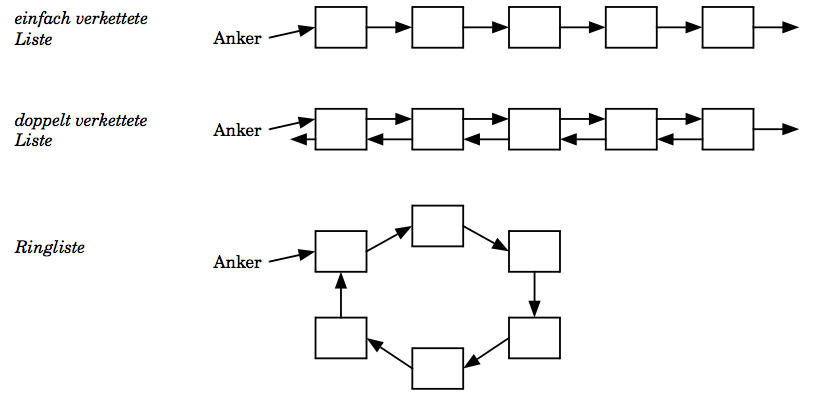
\includegraphics[scale=0.4]{listen.png}
\end{center}

\lstinputlisting[language=java,caption=einfache Linked List,style=JavaStyle]{linked_list.java}


\subsection{Stack}
Der Stack ist eine dynamische Datanstruktur bei der man nur auf das oberste Element des Stabels zugreifen (top), ein neues Element auf den Stabel legen (push) oder das oberste Element des Stapels entfernen (pop) kann.
\lstinputlisting[language=java,caption=Implementierung eines Stacks,style=JavaStyle]{stack.java}

\subsection{Erweiterte Liste}
Dies ist mal eine m�gliche und vor allem nur teilweise Implementierung einer doppelt verlinkten Liste. Die Implementierung des Iterators und der sortierung sind ausgeklammert in Unterkapitel.
\lstinputlisting[language=java,caption=Liste mit Iterator,style=JavaStyle]{advanced_list.java}

\subsubsection{Iterators}
Die Schnittstelle java.util.Iterator, erlaubt das Iterieren von Containerklassen. Jeder Iterator stellt Funktionen namens next(), hasNext() sowie eine optionale Funktion namens remove() zur Verf�gung. Der folgende ListIterator stellt auch noch Funktionen f�r r�ckwertsiterieren zur Verf�gung, sowie die M�glichkeit den aktuellen Index abzufragen. Zudem kann damit noch direkt �ber den Iterator Elemente eingef�gt oder ersetzt werden.

\lstinputlisting[language=java,caption=Iterators,style=JavaStyle]{linked_list_iterators.java}

\subsubsection{Merge Sort}
\lstinputlisting[language=java,caption=Merge Sort,style=JavaStyle]{linked_list_mergesort.java}

\subsection{Skip-Liste}
Die Skip-Liste ist eine sortierte, einfach verkettete Liste, die uns aber ein schnelleres Suchen von Elementen in der Datenstruktur erlaubt. In einer sortierten, verketteten Liste m�ssen wir jedes Element einzeln durchlaufen bis wir das gew�nschten Element gefunden haben. Wenn wir nun aber in der sortierten Liste auf jedem zweiten Element eine zus�tzliche Referenz auf zwei Elemente weiter hinten setzen, dann reduziert sich die Anzahl zu besuchender Elemente auf einen Schlag um rund die H�lfte. Genau betrachtet mu?ssen wir nie mehr als $(n/2) + 1$ Elemente besuchen (n ist die L�nge der Liste). 
\begin{center}
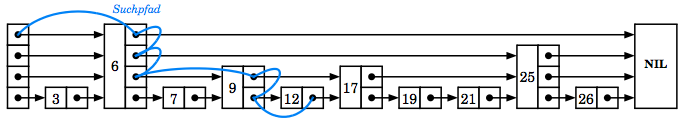
\includegraphics[scale=0.65]{skip_liste.png}
\end{center}

\subsubsection{Beispiel}
\lstinputlisting[language=java,caption=Skip List,style=JavaStyle]{skip_liste.java}

\newpage
\section{B�ume}
Ba?ume sind verallgemeinerte Listenstrukturen. Ein Element, �blicherweise spricht man von Knoten (node), hat nicht, wie im Falle linearer Listen, nur einen Nachfolger, sondern eine endliche, begrenzte Anzahl von S�hnen. In der Regel ist einer der Knoten als Wurzel (root) des Baumes ausgepr�gt. Das ist zugleich der einzige Knoten ohne Vorg�nger. Jeder andere Knoten hat einen (unmittelbaren) Vorg�nger, der auch Vater des Knotens genannt wird. Eine Folge $p_0$, ..., $p_k$ von Knoten eines Baumes, die die Bedingung erf�llt, dass $p_i+1$ Sohn von $p_i$ ist f�r $0 \leq i <$ k, heisst Pfad (path) mit L�nge k, der $p_0$ mit $p_k$ verbindet. Jeder von der Wurzel verschiedene Knoten eines Baumes ist durch genau einen Pfad mit der Wurzel verbunden.
\begin{center}
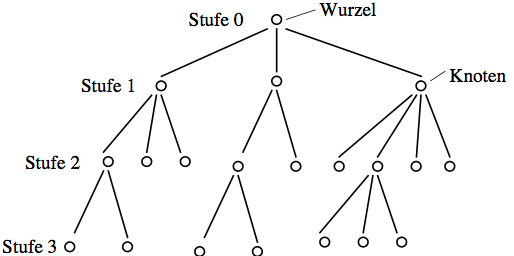
\includegraphics[scale=0.65]{tree.png}
\end{center}

\subsection{Bin�re Suchb�ume}
Ein bin�rer Suchbaum ist ein geordneter Baum mit Ordnung d = 2. In jedem Knoten wird ein Suchschl�ssel so abgespeichert, dass alle Suchschl�ssel des linken Teilbaums des Knotens kleiner und alle Suchschl�ssel des rechten Teilbaums des Knotens gr�sser sind. Das heisst, dass an jedem Knoten alle kleineren Suchschl�ssel �ber den linken Sohn und alle gro?sseren Suchschl�ssel �ber den rechten Sohn erreicht werden.\\
Die so geordneten Knoten in einem balancierten bin�ren Suchbaum erlauben ein schnelles Suchen. Der maximale Suchaufwand h�ngt direkt von der H�he des Baumes ab und w�chst nur logarithmisch mit der Anzahl der Knoten im Baum.
	
\subsubsection{Traversieren}
Das Durchlaufen kann auf mindestens drei verschiedene Arten erfolgen: Preorder, Inorder, Postorder.
\begin{description}
	\item[Inorder] \hfill \\
		1. traversiere den linken Teilbaum des Knotens v; 2. besuche den Knoten v; 3. traversiere den rechten Teilbaum des Knotens v.
	\item[Preorder] \hfill \\
		Bei Preorder wird zuerst Knoten v besucht, dann erst 99 der linke Teilbaum von v in Preorder und anschliessend noch der rechte Teilbaum von v in Preorder durchlaufen.
	\item[Postorder] \hfill \\
		Hier wird zuerst der linke Teilbaum von v, dann der rechte Teilbaum von v und erst zum Schluss der Knoten v besucht.
\end{description}

\subsection{Balancierte B�ume}
% Inhalt Ende
\end{document}